% !TeX spellcheck = cs_CZ
\begin{example}\label{TEO:exam017}
  \textbf{Návrh cívky pro výkonový rezonanční obvod:}
  \newline Požadované parametry:
  \begin{itemize}[noitemsep]
    \item \(L =       \qty{0.32}{\micro\henry}\),
    \item \(I_{max} = \qty{147}{\ampere}\),
    \item \(I_{ef}  = \qty{56}{\ampere}\),
    \item \(f =       \qty{180}{\kilo\hertz}\)
  \end{itemize}
  
  \emph{Řešení:}
  Na cívku jsou kladeny velké nároky. Musí mít požadovanou indukčnost, nesmí být přesycována ani 
  při špičkovém proudu (který je značný), dále je důležitý co největší činitel jakosti (malé 
  ztráty) při daném kmitočtu.
  
  Uspokojivým řešením je cívka navinutá na uzavřeném hrníčkovém jádře. Nejsou u ní problémy s 
  vnějším rozptylovým magnetickým tokem, avšak díky velké magnetické vodivosti jádra bude nutno 
  zajistit velkou vzduchovou mezeru (viz. dále, algoritmus návrhu cívky). Počet závitů a tím délka 
  vodiče vinutí je relativně malá oproti cívce vzduchové, což vede ke snížení ohmických ztrát. 
  Snížení ohmických ztrát způsobených skinefektem se dosáhne použitím svazku tenkých izolovaných 
  (lakovaných) vodičů pro vinutí cívky. To vše přispěje k dosažení maximálního činitele jakosti.
  \emph{Postup návrhu cívky:}
  \begin{enumerate}[noitemsep]
    \item \textbf{Zvolíme jádro}: hrníček \texttt{P42x29} z materiálu \texttt{H21} fy 
          Pramet Šumperk. Katalog: Průřez jádra \(S_c = \qty{265}{\square\mm}\). Magnetická 
          vodivost jádra \(A_L = \qty{8980}{\nano\henry}\) (bez vzduchové mezery).
          
           {\centering
            \captionsetup{type=figure}
            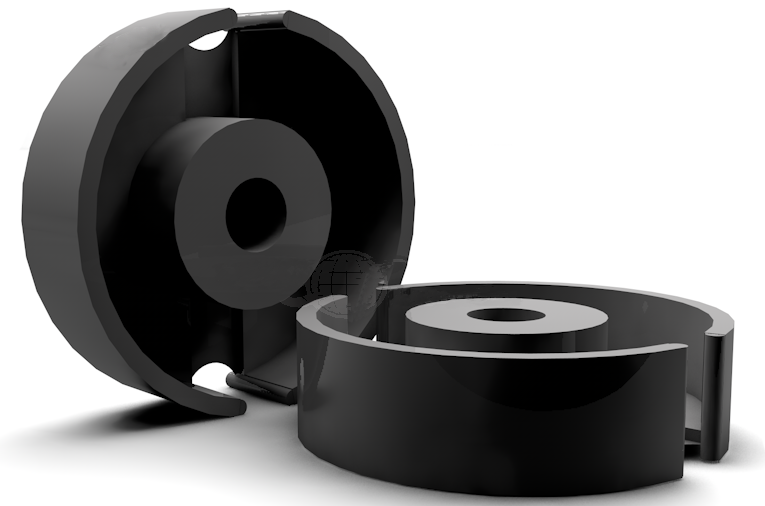
\includegraphics[width=0.35\linewidth]{pot_core.png}
            \captionof{figure}{Hrníčkové jádro}
            \label{ES:fig_001}
          \par}
          
          Kvůli redukci ztrát v jádře volíme dovolené maximální sycení \(B_m\) pouze 
          \qty{0.1}{\tesla} (dovolená hodnota pro daný materiál je cca \qty{0.35}{\tesla}, 
          závisí na teplotě).
    \item Potřebný počet závitů cívky dle:
          \begin{equation*}
            N = \frac{LI_{max}}{B_{max}S}
              = \frac{\num{.32d-6}\cdot\num{147}}{\num{.1}\cdot\num{265d-6}}
              = \num{1.78}
          \end{equation*}
          Pro snadnou realizaci voleno \(N = \num{1.5}\) závitu. Maximální indukce pak bude 
          asi \(\qty{0,12}{\tesla}\).
    \item Vzduchová mezera v jádře musí mít dle (\ref{ES:eq_009}) délku:
          \begin{align*}
            l_v &= \left(\frac{N^2}{L}-\frac{1}{\Lambda}\right)\mu_0           \\
                &= \left(\frac{\num{1.5}^2}{\num{.32d-6}}-
                   \frac{1}{\num{8980d-9}}\right)\num{4\pi d-7}\,\num{265e-6}  \\
                &= \qty{2.3}{\mm}
          \end{align*}
          Realizujeme ji zabroušením středního sloupku jádra.
          Průřez mědi svazku tvořícího vodič vinutí pak musí být:
          \begin{equation*}
            S_v = \frac{I_{ef}}{J} = \frac{\num{56}}{\num{2.3}} = \qty{24.6}{\square\mm}
          \end{equation*}
          Hloubka vniku při kmitočtu \(f = \qty{180}{\kHz}\) bude:
          \begin{equation*}
            \delta = \frac{\num{75}}{\sqrt{f}} 
                   = \frac{\num{75}}{\sqrt{\num{180d3}}} = \qty{.18}{\mm}
          \end{equation*}
          Průměr jednoho drátu svazku tedy smí být maximálně \(2\delta\) tj. \qty{.36}{\mm}. 
          Použijeme vodič \texttt{CuL} s průměrem \qty{.355}{\mm}. Průřez drátu je dán vzorcem 
          \(S_1 = \frac{1}{4}\pi d^2\). Z poměru \(\frac{S_v}{S_1}\) určíme počet vodičů  ve 
          svazku:
          \begin{equation*}
            n = \frac{4S_v}{\pi d^2} 
              = \frac{\num{4}\cdot\num{24.6}}{\pi\cdot\num{.355}^2}
          \end{equation*}
    \item Průměr takto vytvořeného svazku i s vnější izolací bude odhadem asi \qty{7.5}{\mm}.
          Rozměry okénka jádra jsou \(\num{20.3}\times\qty{8.95}{\mm}\). Při tloušťce 
          kostřičky cca \qty{1.5}{\mm} lze počítat s okénkem pro vinutí o rozměrech 
          \(\num{17.3}\times\qty{7.45}{\mm}\). Průřez tohoto okna je: 
          \begin{equation*}
            S_{okno} = \num{17.3}\cdot\qty{7.45}{\square\mm} = \qty{128}{\square\mm}
          \end{equation*}
          Vinutí má \num{1.5} závitu. To znamená, že v jedné polovině obvodu jsou v daném 
          okénku závity dva. Ve jmenované obvodu je tedy činitel plnění:
          \begin{equation*}
            k_{pl} = \frac{2S_v}{S_{okno}} 
                   = \frac{\num{2}\cdot\num{24.6}}{\num{128}} = \num{.38}
          \end{equation*}
          To je reálná hodnota i při našem způsobu vinutí (nikoliv volné vodiče do vrstev, 
          ale \num{1.5} závitu silným předem vyrobeným svazkem s vnější izolací). Vinutí se 
          dobře vtěsná, aniž by přitom zůstal velký prostor nevyužit. To je důkazem správné 
          počáteční volby velikosti jádra.
    \item Výpočet odporu vinutí:
          Měrný odpor mědi při předpokládané teplotě vinutí \qty{80}{\celsius}:
          \begin{align*}
            \varrho_{80} &= \varrho_{20}(1+\alpha\Delta t)  \\
                         &= \num{.0178}(1+ \num{4d-3}\cdot60)
                          = \qty{.22}{\ohm\square\mm\per\m}
          \end{align*}
          Délka jednoho závitu cívky: cca \qty{126}{\mm}\newline
          Délka celého vinutí i s přívody: \(l=\qty{250}{\mm}\) \newline
          Odpor vinutí při  \qty{80}{\celsius}:
          \begin{equation*}
            R = \varrho_{80}\frac{l}{S_v} 
              = \num{.022}\frac{\num{.25}}{\num{24.6}} = \qty{2.24d-4}{\ohm}
          \end{equation*}
          Ohmické ztráty na vinutí při \(I_{ef}\):
          \begin{equation*}
            P_{Cu} = R_{Cu}I_{ef}^2 = \num{2.24d-4}\cdot\num{56}^2 = \qty{.7}{\watt}
          \end{equation*}
          Hysterezní ztráty v jádře:\newline
          Katalogový údaj pro dané jádro: \(P_{h0} = \qty{3}{\watt}\) při \(f_0 = 
          \qty{15}{\kilo\Hz}\) a \(B_0 = \pm\qty{.2}{\tesla}\)
          \begin{align*}
            P_{h}   &= \frac{1}{4}P_{h0}\left(\frac{B}{B_0}\right)^2\frac{1}{T_{ekv}\cdot f} \\
                    &= \frac{1}{4}\cdot\num{3}\left(\frac{\num{.12}}{\num{.2}}\right)^2
                       \frac{1}{\num{12.7d-6}\cdot\num{15d3}} = \qty{1.4}{\watt}              \\
            \shortintertext{Celkové ztráty:}
            P_{tot} &= P_{Cu} + P_{h} = \num{.7} + \num{1.4} = \qty{2.1}{\watt}
          \end{align*}
  \end{enumerate}
\end{example}
